% !TEX TS-program = XeLaTeX
\documentclass[a4paper]{article}

% https://tex.stackexchange.com/questions/172234/define-and-set-length-in-one-command
\newcommand{\deflen}[2]{%      
    \expandafter\newlength\csname #1\endcsname
    \expandafter\setlength\csname #1\endcsname{#2}%
}

\newcommand{\goldenratio}{1.618}

\deflen{horizontalmarg}{1.0cm}
\deflen{verticalmarg}{1.618cm}

\usepackage[top=\the\verticalmarg, bottom=\the\verticalmarg, 
  left=\the\horizontalmarg, right=\the\horizontalmarg]{geometry}



\newlength{\lowerbaroffset}
\setlength{\lowerbaroffset}{0.8cm}

\newlength{\localpwidth}

\newlength{\contentswidth}
\setlength{\contentswidth}{\dimexpr(\paperwidth-2\horizontalmarg)}
\newlength{\contentsheight}
\setlength{\contentsheight}{\dimexpr(\paperheight-2.01\verticalmarg)}


\newlength{\halfwidth}
\setlength{\halfwidth}{\dimexpr(0.5\contentswidth)}

\usepackage{fontspec,lipsum}

% Just to display the page bounds
\newcommand{\helperrect}{\draw[color=gray] (0,0) rectangle (\the\contentswidth, \the\contentsheight);}

% A4: 21.0 × 29.7
\pagenumbering{gobble}
\setmainfont[Path=../fonts/]{Muli-Regular.ttf}
\usepackage{tikz}

% TODO: See if Melissa provided some design document
% with precise specs of margins, font sizes, etc.

\begin{document}
\noindent
\begin{tikzpicture}[x=1cm, y=1cm]
\definecolor{anemored}{rgb} {1.00,0.129,0.247}
\helperrect


\setlength{\localpwidth}{10cm}


%\node[inner sep=0pt, anchor=north west] (anemobox) at (0cm,\the\contentsheight) {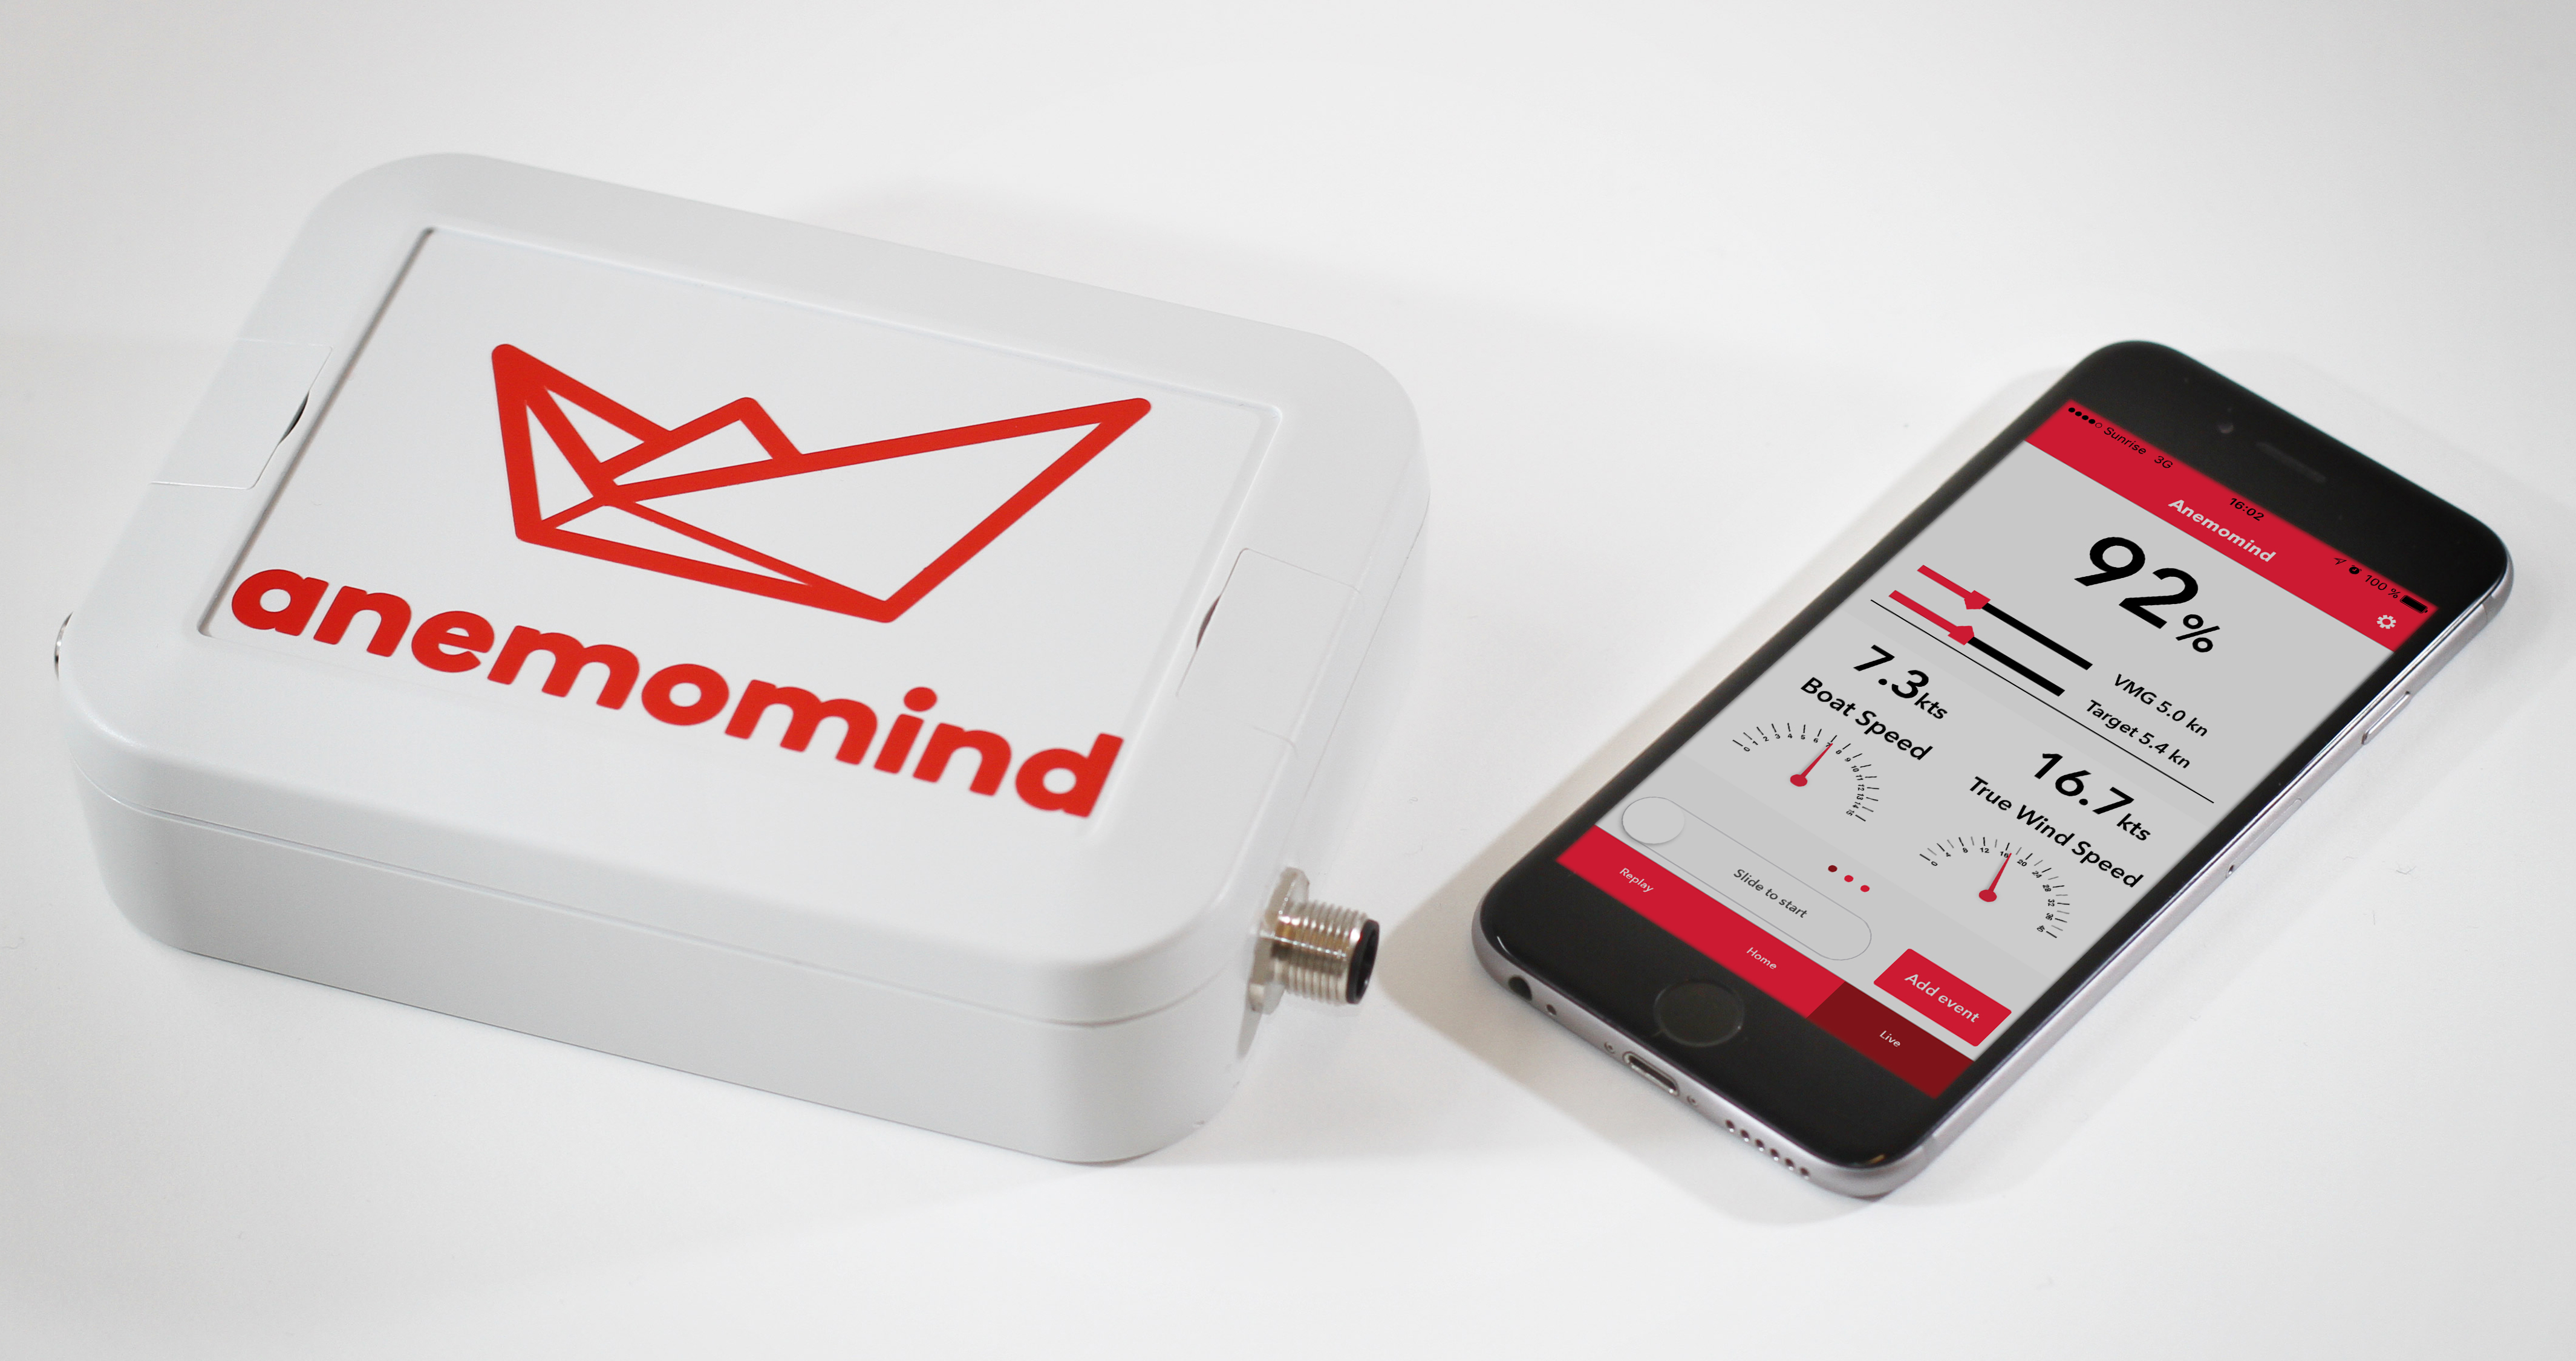
\includegraphics[width=\the\halfwidth]{../images/anemobox10.jpg}};

%% \foreach \bound in {north,south,west,east,45} {
%%       \node[anchor=\bound] at (current page.\bound) {I am \bound-bound...};
%%   }
  \node[anchor=north west, color=anemored] at (0, \the\contentsheight) {\Large Specifications!};
  \draw[color=anemored, line width=0.25mm] (0, \the\dimexpr(\contentsheight-\lowerbaroffset)) -- (\the\localpwidth, \the\dimexpr(\contentsheight-\lowerbaroffset));
%\node[draw=none] at (0,0) {some text};
%\node[draw] at (0,0) {some text};

\end{tikzpicture}
\end{document} 

